\documentclass[12pt,french]{book}
\usepackage[utf8]{inputenc}
\usepackage{tgpagella} % Palatino text only
\usepackage{mathpazo}  % Palatino math & text
\usepackage[left=1.5in,right=1.5in,top=1.5in,bottom=1.5in]{geometry}
% \linespread{1.5}
% \usepackage[super,comma,sort]{natbib}
\usepackage[round,sort&compress]{natbib}
\usepackage{url} % [hyphens]
\usepackage[hyperpageref]{backref} % back references biblio. Needs latexmk at compilation.
\usepackage[pagebackref]{hyperref}
% \usepackage{multibib} % incompatible with backref
\hypersetup{
  colorlinks=true, % breaklinks=true,
  urlcolor=purple,    % color of external links
  linkcolor=blue,  % color of toc, list of figs etc.
  citecolor=violet,   % color of links to bibliography
}
\usepackage{bm}
\usepackage{indentfirst}
\usepackage{tocbibind}
\setcitestyle{aysep={}} 
\usepackage{amsmath}
\usepackage{amssymb}
\usepackage{eurosym}
\usepackage{amsfonts}
\usepackage{enumerate}
\usepackage{babel}
\usepackage{caption}
\usepackage{supertabular}
\usepackage{tabularx}
\usepackage{float}
\usepackage{dsfont}
\usepackage{fancyvrb}
\usepackage{verbatim}
\usepackage{enumitem}
\usepackage{setspace}
\usepackage{comment}
\usepackage{subcaption}
\usepackage{graphicx}
\usepackage{tikz}
\usepackage{gensymb}
\usepackage{textcomp}

\usepackage{tabulary}
\usepackage{tabularx}
\usepackage{booktabs}
\usepackage{fullpage}
\usepackage{morefloats}
\usepackage{makecell}
\usepackage{lscape}
\usepackage{pdflscape}
\usepackage{longtable}
\usepackage{rotating}
\usepackage{fancyhdr}
\usepackage{tocloft}
\usepackage{titletoc}
\usepackage[export]{adjustbox}
\usepackage[anythingbreaks]{breakurl} % for links
\usepackage{multicol}
\newsavebox\ltmcbox % For net gain table over two columns
%\usepackage[nomarkers,figuresonly]{endfloat} % Figures at the end
%\usepackage[section,below]{placeins} % Floats placed in the section they appear in.
\renewcommand{\floatpagefraction}{.9}

% \renewcommand{\thechapter}{\Roman{chapter}}

\title{Un plan mondial pour le climat \\et contre l'extrême pauvreté} 
% Pour une révolution fiscale: 42k mots, 290 mots par page.

\author{Adrien Fabre\footnote{CNRS, CIRED. E-mail: adrien.fabre@cnrs.fr.}} 

\date{\today} 

\begin{document}

\maketitle

\tableofcontents

\chapter{Un statu quo insupportable}
% Un statu quo insupportable : l'extrême pauvreté, le changement climatique (chiffres, constat)

Plusieurs fléaux affligent l'humanité. Dans ce livre, nous nous préoccupons de deux d'entre eux : le changement climatique et l'extrême pauvreté. La lenteur des progrès effectués est une honte pour l'humanité, qui ne semble pas se soucier des personnes vulnérables ni des générations futures. Le constat est insupportable.

\section{Le changement climatique}

Le climat est un système complexe, mais les travaux du GIEC ont prouvé qu'on pouvait l'approximer avec une règle simple : le réchauffement climatique est proportionnel aux émissions de CO$_\text{2}$ cumulées depuis la révolution industrielle\footnote{La Figure SPM.10 in \citet{ipcc_climate_2021} montre qu'un degré de plus correspond à 2~000 GtCO$_\text{2}$.}. Pour mettre fin au réchauffement climatique dû à l'accumulation de CO$_\text{2}$ dans l'atmosphère, il faut donc atteindre la neutralité carbone. En d'autres termes, il faut amener les émissions de CO$_\text{2}$ à zéro --- ou plus exactement zéro net, des émissions résiduelles pouvant être compensées par une captation équivalente grâce à la reforestation ou la séquestration artificielle du carbone. La température à laquelle l'humanité choisit de stabiliser le climat détermine le budget carbone, c'est-à-dire les émissions qu'il nous reste à émettre. Par exemple, pour avoir deux chances sur trois de limiter le réchauffement à +2\textdegree{}C, le budget carbone est de 1~000 milliards de tonnes (Gt) de CO$_\text{2}$ à partir de 2024\footnote{cf. Table SPM.2 in \citet{ipcc_climate_2021}. La probabilité vient du fait que les modèles climatiques comportent une marge d'erreur sur la température atteinte par un budget carbone donné.}. Le budget carbone pourrait être respecté en réduisant linéairement les émissions de CO$_\text{2}$, en partant de leur valeur actuelle de 38 Gt jusqu'à zéro en 2077. 

Si, au contraire, les émissions continuent de croître, le réchauffement pourrait atteindre +4\textdegree{}C en 2100, et jusqu'à +7-8\textdegree{}C entre 2300 et 5000\footnote{\citet{montenegro_long_2007}}. La fonte de l'Antarctique pourrait élever le niveau de la mer de 15 mètres d'ici 2500 et submerger d'ici 2300 des zones côtières où vivent actuellement près d'un milliard de personnes\footnote{\citet{deconto_contribution_2016,kopp_evolving_2017}}. De vastes zones de Chine, d'Asie du Sud et du Moyen-Orient seraient rendues inhabitables au XXII$^\text{e}$ siècle du fait d'une combinaison létale de température et d'humidité\footnote{\citet{pal_future_2016,im_deadly_2017,kang_north_2018}}. Même dans un scénario d'émissions moins extrême, avec une température de +2\textdegree{}C en 2100, le niveau de la mer submergerait (en l'absence de digues) des zones où vivent actuellement 250 millions de personnes\footnote{\citet{kulp_new_2019}}. De manière générale, nos infrastructures (et nos usages des sols) sont adaptées au climat actuel et le changement climatique en rendra de nombreuses obsolètes, lorsqu'elles ne seront pas tout simplement détruites. Pour résumer, la continuation des émissions de gaz à effet de serre mettrait en péril de multiples pans de la société, multipliant les sécheresses, réduisant les rendements agricoles, accroissant la probabilité de conflit violent, et entraînant d'importants déplacements de population\footnote{Ce paragraphe reprend des éléments du préambule de ma thèse \citep{fabre_is_2020}, et repose sur de nombreux travaux \citep{burke_warming_2009,cattaneo_human_2019,carleton_social_2016,dell_temperature_2012,elliott_constraints_2014,schlenker_robust_2010,moore_new_2017}.}. 

% Climat et distribution
% Net zéro est possible

\section{L'extrême pauvreté} % Les pauvres ont faim / La faim de l'extrême pauvreté

La Banque mondiale définit l'extrême pauvreté par une consommation inférieure à 2\$ par jour (en parité de pouvoir d'achat\footnote{Le seuil de 2\$ est exprimé en parité de pouvoir d'achat (2,15\$ en dollar constant de 2017 pour être exact) : il correspond à ce que 2\$ permet d'acheter aux États-Unis. Dans un pays comme l'Inde, il faut ainsi moins de 1\$ pour se procurer l'équivalent de 2\$ aux États-Unis.}). % https://data.worldbank.org/indicator/NY.GDP.PCAP.KD?end=2021&locations=EU-ZG-XD-XM-1W-IN-US-CD-BI-LU-CN&start=2021&view=bar / https://data.worldbank.org/indicator/NY.GDP.PCAP.PP.KD?end=2021&locations=EU-ZG-XD-XM-1W-IN-US-CD-BI-LU-CN&start=2021&view=bar
Ce seuil permet de satisfaire les besoins nutritionnels minimaux\footnote{\citet{allen_absolute_2017-1} calcule que, dans les pays à bas revenus, le seuil d'extrême pauvreté permet de payer 3 m² dans un logement chauffé à 15\textdegree{}C ainsi qu'un régime alimentaire constitué uniquement d'huile et d'une céréale (parfois complété par des lentilles), qui assure un apport journalier de 2100 kcalories, 50 g de protéines et 34 g de lipides.}. Ainsi, le nombre de personnes en situation d'extrême pauvreté recoupe celui des 700 millions de personnes sous-alimentées\footnote{\citet{fao_state_2023}, \href{https://data.worldbank.org/indicator/SI.POV.DDAY?end=2019&locations=MW-1W&start=1990&view=chart}{Banque mondiale}.}. 

Bien que la proportion d'humains vivant avec moins de 2\$ par jour ait été divisée par quatre dans les trente dernières années, cela concerne encore deux tiers de la population dans un pays comme le Malawi. En fait, avec l'augmentation de la population, il y a davantage d'Africains extrêmement pauvres aujourd'hui qu'il y a trente ans. Si l'extrême pauvreté s'est réduite durant la période, c'est uniquement grâce au développement de l'Asie, et en particulier de la Chine. % https://ourworldindata.org/poverty?insight=hundreds-of-millions-will-remain-in-extreme-poverty-on-current-trends#key-insights

La Chine a désormais un PIB par habitant autour de la moyenne mondiale, soit 960\euro{} par mois. % world current GDP pc 2022 (current $): 12703 
En comparaison, le PIB par habitant est trois fois plus élevé dans les pays à hauts revenus et dix fois plus faible dans les pays à bas revenus. L'écart de niveau de vie est difficile à exagérer. En effet, un transfert de seulement 1\% du PIB des pays à hauts revenus (1,2 milliard de personnes) doublerait mécaniquement le revenu national des pays à bas revenus (700 millions de personnes). 

\begin{figure}[h!]
  \caption{PIB par habitant par rapport à la moyenne mondiale, ajustés en parité de pouvoir d'achat (2021, Banque mondiale). %Selected GDP per capita in PPP relative to the World's (2021, World Bank).
  }\label{fig:GDPpc}
  \makebox[\textwidth][c]{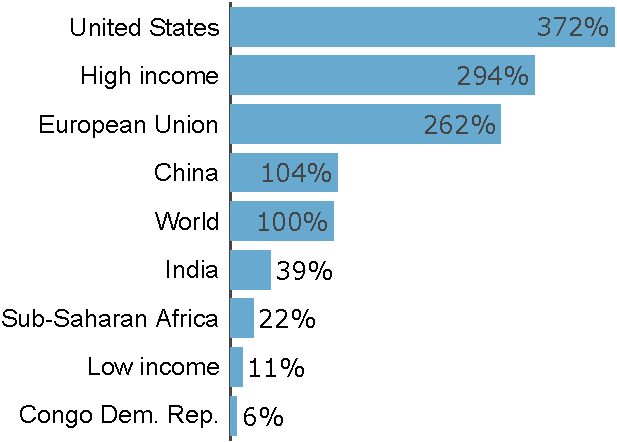
\includegraphics[width=.56\textwidth]{../figures/policies/GDP_pc_PPP_few.pdf}} % https://data.worldbank.org/indicator/NY.GDP.PCAP.PP.CD?contextual=default&end=2021&locations=EU-ZG-XD-XM-1W-IN-US-CD-BI-LU-CN&start=2021&view=bar
\end{figure}

\chapter{La nécessité de redistribution mondiale}

Qu'elle soit religieuse, philosophique ou intuitive, la morale prescrit généralement des transferts des personnes à hauts revenus vers les personnes à bas revenus, et donc des pays à hauts revenus vers les pays à bas revenus. C'est le cas de l'utilitarisme, la théorie éthique de référence utilisée en économie. L'utilitarisme attribue le même poids à chaque personne et considère ainsi le transfert d'un euro d'une personne riche à une personne pauvre, puisqu'un euro procurera plus de satisfaction à cette dernière. D'après la théorie de la taxation optimale, ce raisonnement est valable tant qu'une augmentation des prélèvements n'incite pas les plus riches à réduire, expatrier ou dissimuler leur activité au point de diminuer les recettes obtenues. En tenant compte de ces effets, des économistes ont calculé qu'un système fiscal optimal reduirait drastiquement les inégalités entre pays et procurerait un revenu minimum de 250\$ par mois au niveau mondial\footnote{Dans ces calculs, \citet{kopczuk_limitations_2005} se limitent à un taux unique (une \textit{flat tax}) et ne s'autorisent pas un barème progressif. Sans cette restriction, le véritable optimum serait encore plus redistributif.}. Pour rationaliser la faiblesse des transferts internationaux, la théorie de la taxation optimale nécessite d'attribuer un poids 2~000 fois plus élevé à un Américain qu'à un Congolais (ou bien, d'attribuer une valeur 100 fois supérieure à l'Américain et de considérer que seul un vingtième de l'argent transféré arrivera à son destinataire, le reste étant détourné par la corruption). %de distordre les poids de sorte que la satisfaction d'un Américain vaille autant que celle de 2~000 Malgaches. 

Au-delà des considérations éthiques, la redistribution mondiale a des fondements juridiques. En 2015, l'ensemble des pays a adopté les Objectifs de développement durable (ODD), au premier rang duquel se trouve l'élimination de l'extrême pauvreté d'ici à 2030. Or, les pays à bas revenus n'ont pas les ressources domestiques suffisantes pour éliminer l'extrême pauvreté. En effet,  dans les 19 pays les plus pauvres, exproprier tous les revenus à partir de 13\$ par jour ne suffirait pas à financer des transferts suffisants pour faire passer leurs 700 millions d'habitants au-dessus de 2\$ par jour d'ici à 2030. Même en faisant l'hypothèse très optimiste d'une croissance du revenu moyen de 7\% par an d'ici à 2030% (soit le maximum observé dans le monde dans les cinq années qui ont précédé la Covid)
, exproprier tous les revenus au-delà de 7\$ par jour ne suffirait pas à éliminer l'extrême pauvreté dans un pays tel que Madagascar\footnote{Ces calculs sont inspirés de \citet{bolch_arithmetics_2022}, reposent sur les données \textit{Poverty and Inequality Platform} de la Banque mondiale, et sont reproductibles sur \href{https://github.com/bixiou/domestic\_poverty\_eradication/code\_poverty/main.R}{github.com/bixiou/domestic\_poverty\_eradication}.}. En d'autres termes, il est impossible d'atteindre le premier ODD sans transferts internationaux. Plus généralement, 12 ODD sur les 17 concernent la pauvreté, les inégalités et le changement climatique. Si les pays à bas revenus n'ont déjà pas les ressources nécessaires pour éliminer l'extrême pauvreté (estimées à 0,1\% du PIB mondial), % 2019 poverty gap = 2.6% of $2.15 / world GDP of 16865 https://data.worldbank.org/indicator/SI.POV.GAPS
il va sans dire qu'une redistribution internationale est nécessaire pour développer des services de santé, d'éducation, une énergie décarbonée, et plus généralement atteindre l'ensemble des ODD.

% Si les pays de l'OCDE tenaient leur promesse d'allouer 0,7\% de leur PIB à l'aide publique au développement, dont 0,2\% du PIB pour les pays les moins avancés, les ODD pourraient être remplis\footnote{Cf. \citet{sdsn_sdg_2019}.}. 
% Flux dans l'autre sens
% promesse ODA + conditionalité CDNs

% ODA for LDCs: only Luxembourg is above the objective of 0.2% of GNI (SDG 17.2) https://data.worldbank.org/indicator/DC.ODA.TLDC.GN.ZS?locations=US-GR-LU-SE-GB&most_recent_value_desc=true
% 19 pays (570M en 2022, 700M en 2030) ne pourraient pas éradiquer l'extrême pauvreté même en expropriant tous les revenus au-delà de 13$/jour. Pays comme la RDC ne pourrait pas mettre fin à l'extrême pauvreté en 2030, même avec une croissance de 6% et en expropriant tous les revenus au-delà de 7$/jour.

% Addressing global poverty, inequalities and climate change are at the heart of the universally agreed Sustainable Development Goals (SDG). % 12 out of  17
% It has been pointed out that low-income countries generally do not have enough domestic resources to eliminate the poverty gap in the short run.\cite{bolch_arithmetics_2022} % In other words, it would hardly be possible to achieve the first SDG and end extreme poverty by 2030 without international transfers. => Careful, Bolch use a poverty line above the SDG one.



\chapter{Les grands principes du Plan mondial pour le climat}
% Le plan mondial pour le climat : les grands principes (description de la mesure, des trajectoires)

\chapter{Les détails du Plan}
% Le plan mondial pour le climat : les détails (implémentation, mécanismes de participation)

\chapter{Un transfert massif vers les pays du Sud}
% Le plan mondial pour le climat : les effets distributifs (carte des pays gagnants et perdants)

\chapter{Un Plan largement soutenu}

\citet{fabre_global_2023}
% Un plan largement soutenu (soutien majoritaire dans 20 pays, avantage électoral aux partis de gauche qui l'incluraient dans leur programme, consensus en faveur de la répartition égalitaire de l'effort de décarbonation)

\chapter{Un pas vers un monde soutenable}
% Un pas vers un monde soutenable (le Plan n'est pas suffisant, il doit être complémenté d'autres mesures climatiques (nationales, sectorielles), d'autres mesures de redistribution mondiale (impôt sur la fortune), et l'objectif de long terme doit être d'assurer les conditions nécessaires au bien-être à chaque humain)

\chapter{L'appel pour la redistribution mondiale}
% L'appel pour la redistribution mondiale (description de l'activité de Global Redistribution Advocates, lien vers la lettre ouverte aux dirigeants pour la redistribution mondiale - que nous prévoyons de publier dans les grands journaux type The Guardian, Le Monde..., appel à une manifestation mondiale en soutien à cet appel le 1er décembre 2024 lors de la COP29).

\chapter{Foire Aux Questions}


% \begin{center}
% {\textbf{\href{https://github.com/bixiou/global_tax_attitudes/raw/main/paper/book.pdf}{Link to most recent version}}}
% \end{center}

% 0. Préface : j'envisage Thomas Piketty, Jean Tirole, Gaël Giraud ou Esther Duflo pour la version française et Greta Thunberg ou Joseph Stiglitz pour la version anglaise (mais ça reste à définir)
% 1. Un statu quo insupportable : l'extrême pauvreté, le changement climatique (chiffres, constat)
% 2. La nécessité de redistribution mondiale (objectifs de développement durable, justifications théoriques)
% 3. Le plan mondial pour le climat : les grands principes (description de la mesure, des trajectoires)
% 4. Le plan mondial pour le climat : les détails (implémentation, mécanismes de participation)
% 5. Le plan mondial pour le climat : les effets distributifs (carte des pays gagnants et perdants)
% 6. Un plan largement soutenu (soutien majoritaire dans 20 pays, avantage électoral aux partis de gauche qui l'incluraient dans leur programme, consensus en faveur de la répartition égalitaire de l'effort de décarbonation)
% 7. Un pas vers un monde soutenable (le Plan n'est pas suffisant, il doit être complémenté d'autres mesures climatiques (nationales, sectorielles), d'autres mesures de redistribution mondiale (impôt sur la fortune), et l'objectif de long terme doit être d'assurer les conditions nécessaires au bien-être à chaque humain)
% 8. L'appel pour la redistribution mondiale (description de l'activité de Global Redistribution Advocates, lien vers la lettre ouverte aux dirigeants pour la redistribution mondiale - que nous prévoyons de publier dans les grands journaux type The Guardian, Le Monde..., appel à une manifestation mondiale en soutien à cet appel le 1er décembre 2024 lors de la COP29).
% 9. Postface : Foire Aux Questions (description et réponse aux objections habituelles)

% Un plan mondial pour le climat et contre l'extrême pauvreté (version courte illustrée / version longue) :
% - situation pauvreté, csq CC
% - SDGs, justifications redistr. mondiale
% - description GCS, y.c. trajectoires
% - détails implémentation (e.g. Aadhaar)
% - acceptation
% - autres mesures mondiales possibles
% - appel signé par milliers + manif mondiale un an après lancement
% - préface Piketty puis Greta
% - FAQ, y.c. critiques d'une page (et réponses) de Piketty, etc.
% Opuscule Cepremap au pire

% FAQ
% - Les émissions vont augmenter si on distribue un revenu de base et les revenus augmentent
% - Qui paient : entreprises ou consommateurs ?
% - Les quotas profitent aux plus riches qui peuvent s'acheter plus de quotas, les plus pauvres bradent leurs quotas pour des rétributions immédiates en obérant des potentialités pour le futur 
% - pas sûr que ça ait fait ses preuves 
% - il y a certaines pratiques qui vont devoir s'arrêter, il faut interdire
% => Le Plan fournit un cadre qui assure des réductions d'émissions adéquates; qui incite les États à prendre des mesures complémentaires type interdiction; on peut remplacer le système d'échanges de permis par une taxe, c'est équivalent. 
% Pourquoi pas taxe progressive ?
% Problème de la fraude / du monitoring.
% Problème de la transparence sur les implications (les gens réalisent-ils les changements de mode de vie nécessaires ?)
% Qu'est-ce qu'on fait de l'EU ETS? On le laisse en place. 
% Les taxes affectées ne sont-elles pas interdites ? => no, e.g. Chirac tax on flying

% Wealth tax: 
% taxe universelle ? exit tax ?

\renewcommand{\url}[1]{\href{#1}{Link}} % NCCcomment
\bibliographystyle{plainnaturl_clean} % NCCcomment
\bibliography{global_tax_attitudes}

\end{document}